\newcommand{\institut}{}
\newcommand{\fachgebiet}{Regelungstechnik}
\newcommand{\veranstaltung}{Praktikum Grundlagen der Regelungstechnik}
\newcommand{\pdfautor}{Dirk Barbendererde (321 836), Boris Henckell (325 779)}
\newcommand{\autor}{Dirk Barbendererde (321 836)\\ Boris Henckell (325 779)}
\newcommand{\pdftitle}{Praktikum Regelungstechnik  Versuch 1b}
\newcommand{\prototitle}{Praktikum Regelungstechnik \\ Versuch 1b}
\newcommand{\aufgabe}{}

\newcommand{\gruppe}{Gruppe: G1 Di 12-14}
\newcommand{\betreuer}{Betreuer: Christian Schmuck}



\input{../../packages/tu_header_8}


% \lstlistoflistings
\definecolor{darkgray}{rgb}{0.95,0.95,0.95}
\lstset{language=Scilab}
\lstset{inputencoding=utf8}
%\lstset{extendedchars=true} % Umlaute an der richtigen stelle und nicht am Anfang ausgeben
\lstset{backgroundcolor=\color{darkgray}}
\lstset{numbers=left, numberstyle=\tiny, stepnumber=1, numbersep=7pt, breaklines=true}
\lstset{keywordstyle=\color{red}\bfseries\emph}
\lstset{
breaklines,
numbers=left,
frame=single,
xleftmargin=-2cm,
xrightmargin=-1.5cm
}
% enables UTF-8 in source code: (dirty, dirty hack)
\lstset{literate=
    %Deutsch
    {ä}{{\"a}}1 {ö}{{\"o}}1 {ü}{{\"u}}1 {Ä}{{\"A}}1 {Ö}
    {{\"O}}1 {Ü}{{\"U}}1 {ß}{\ss}1
    %Türkisch
    {â}{{\^{a}}}1 {Â}{{\^{A}}}1 {ç}{{\c{c}}}1 {Ç}{{\c{C}}}1 {ğ}{{\u{g}}}1 {Ğ}{{\u{G}}}1 {ı}{{\i}}1 {İ}{{\.{I}}}1 {ö}{{\"o}}1 {Ö}{{\"O}}1 {ş}{{\c{s}}}1
    {Ş}{{\c{S}}}1 {ü}{{\"u}}1 {Ü}{{\"U}}1
    %Polish
    {ą}{{\k{a}}}1 {ć}{{\'c}}1 {ę}{{\k{e}}}1 {ł}{{\l{}}}1 {ń}{{\'n}}1 {ó}{{\'o}}1 {ś}{{\'s}}1 {ż}{{\.z}}1 {ź}{{\'z}}1 {Ą}{{\k{A}}}1 {Ć}{{\'C}}1
    {Ę}{{\k{E}}}1 {Ł}{{\L{}}}1 {Ń}{{\'N}}1 {Ó}{{\'O}}1 {Ś}{{\'S}}1 {Ż}{{\.Z}}1 {Ź}{{\'Z}}1
    %Spanish
    {á}{{\'a}}1 {é}{{\'e}}1 {í}{{\'i}}1 {ó}{{\'o}}1 {ú}{{\'u}}1 {ñ}{{\~n}}1
}

%     \lstinputlisting{./praktikum6.sce}



%---------------------------------------------------------------------
%---------------------------------------------------------------------
%---------------------------------------------------------------------

\section{Vorbereitungsaufgaben}
\begin{quote}
	\hspace{-2em}
	\subsection{Übertragungsfunktion}
    Aufgabe:\\
    Ermittlen Sie die Übertragungsfunktion $G_\omega^{'} (s) = \frac{\Omega(s)}{R_i (s)}$ der nun relevanten
    Regelstrecke, die den unterlagerten Stromregelkreis aus Versuchsteil 1a enthält.\\
	\begin{quote}
	   Zuerst errechnen wir die zweite Regelstrecke $G_2$:\\
	   Der Zustandsvektor $x(t)$ besteht aus der Winkelgeschwindigkeit $\omega(t)$.
        \begin{equation*}
            \begin{split}
                x(t) = 
                    \begin {pmatrix}
                        \omega(t)\\
                    \end{pmatrix}
            \end{split}
        \end{equation*}
        
        Die Stellgröße $u(t)$ besteht aus dem Ankerstrom $i_A(t)$.
        \begin{equation*}
            \begin{split}
                u(t) = i_A (t)
            \end{split}
        \end{equation*}
        
        Als Ausgangsgröße $y(t)$ wird die Winkelgeschwindigkeit $\omega(t)$ genommen.
        \begin{equation*}
            \begin{split}
                y(t) = \omega(t)
            \end{split}
        \end{equation*}
        
        Daraus ergibt sich folgendes Zustandesmodell:
        \begin{equation*}
            \begin{split}
                   \dot{x} &=
                   \begin{pmatrix}
                        \dot{\omega}(t)\\
                   \end{pmatrix}\\ &=
                   \begin{pmatrix}
                        -\frac{c_\mu}{\frac{1}{2}M_s r^2_s + J_m}\\
                   \end{pmatrix} x(t) +
                   \begin{pmatrix}
                       \frac{k_m}{\frac{1}{2}M_sr^2_s + J_m}\\
                   \end{pmatrix} u(t) +
                   \begin{pmatrix}
                       \frac{-1}{\frac{1}{2}M_sr^2_s + J_m}\\
                   \end{pmatrix} m_L(t)\\
                   y(t) &= 
                   \begin{pmatrix}
                        1\\
                   \end{pmatrix} x(t) + 0 \p u(t)
            \end{split}
        \end{equation*}
        
        Daraus folgt folgende Übertragungsfunktion $G_2$:
        \begin{equation*}
        	\begin{split}
        		G_2 (s) = \frac{2351,6287}{0,0178492 + s}
        	\end{split}
        \end{equation*}
        
        Nun können wir $G_\omega^{'}$ berechnen:
	
		\begin{equation*}
        	\begin{split}
        		G_\omega^{'} (s) &= T_1(s) G_2(s) = \frac{G_1 (s) K_1(s)}{1 + G_1 (s) K_1 (s)} G_2 (s)\\ \\
        		&= \frac{475559.23}{3.6095577 + 202.24332s + s^2}
        	\end{split}
        \end{equation*}
		
        
	\end{quote}
	
	\subsection{Regler}
    Aufgabe:\\
    Als Drehzahlregler soll ein PI-Glied\\
    \begin{equation*}
        \begin{split}
            K_\omega (s) = k_\omega \frac{s-s_{0,\omega}}{s}, \hspace{2em} k_\omega, s_{0,\omega} \in \mathbb{R}
        \end{split}
    \end{equation*}
    verwendet werden.
	\begin{quote}
		
		\subsubsection{Sinnvolle Reglerstruktur?}
        Aufgabe:\\
        Begründen Sie, warum diese Reglerstruktur sinnvoll ist.\\
		\begin{quote}
			Die zu regelnde Strecke $G_\omega^{'}$ weist zwei Pole auf der negativen Reellen achse auf und zwar bei:\\
            \\
			$pol_{G\omega^{'}}_1 = - 0,0178492$\\
			\\
			$pol_{G\omega^{'}}_2 = - 202.22547$\\
			\\
			Mit der gewählten Reglerstruktur haben wir die Möglichkeit einerseits den langsamsten Pol der Strecke zu eliminieren
			und zusätzlich einen Integrierenden Anteil in den Regler zu bringen. Dadurch wird eine bleibende Regelabweichung
			verhindert.\\
			Die resultierende Wurzelortskurve des Kreises zeigt, dass für eine gewisse mindestverstärkung der Regelkreis
			asymptotisch stabil bleibt.
		\end{quote}
		
		\subsubsection{Bode-Diagramm}
        Aufgabe:\\
        Der Reglerentwurf soll nach dem Frequenzkennlinienverfahren durchgeführt werden. Zeichnen Sie dafür zunächst
        das Bode-Diagramm von $G_\omega^{'}$.\\   
        \begin{quote}
            \begin{figure}[H]
            \centering
                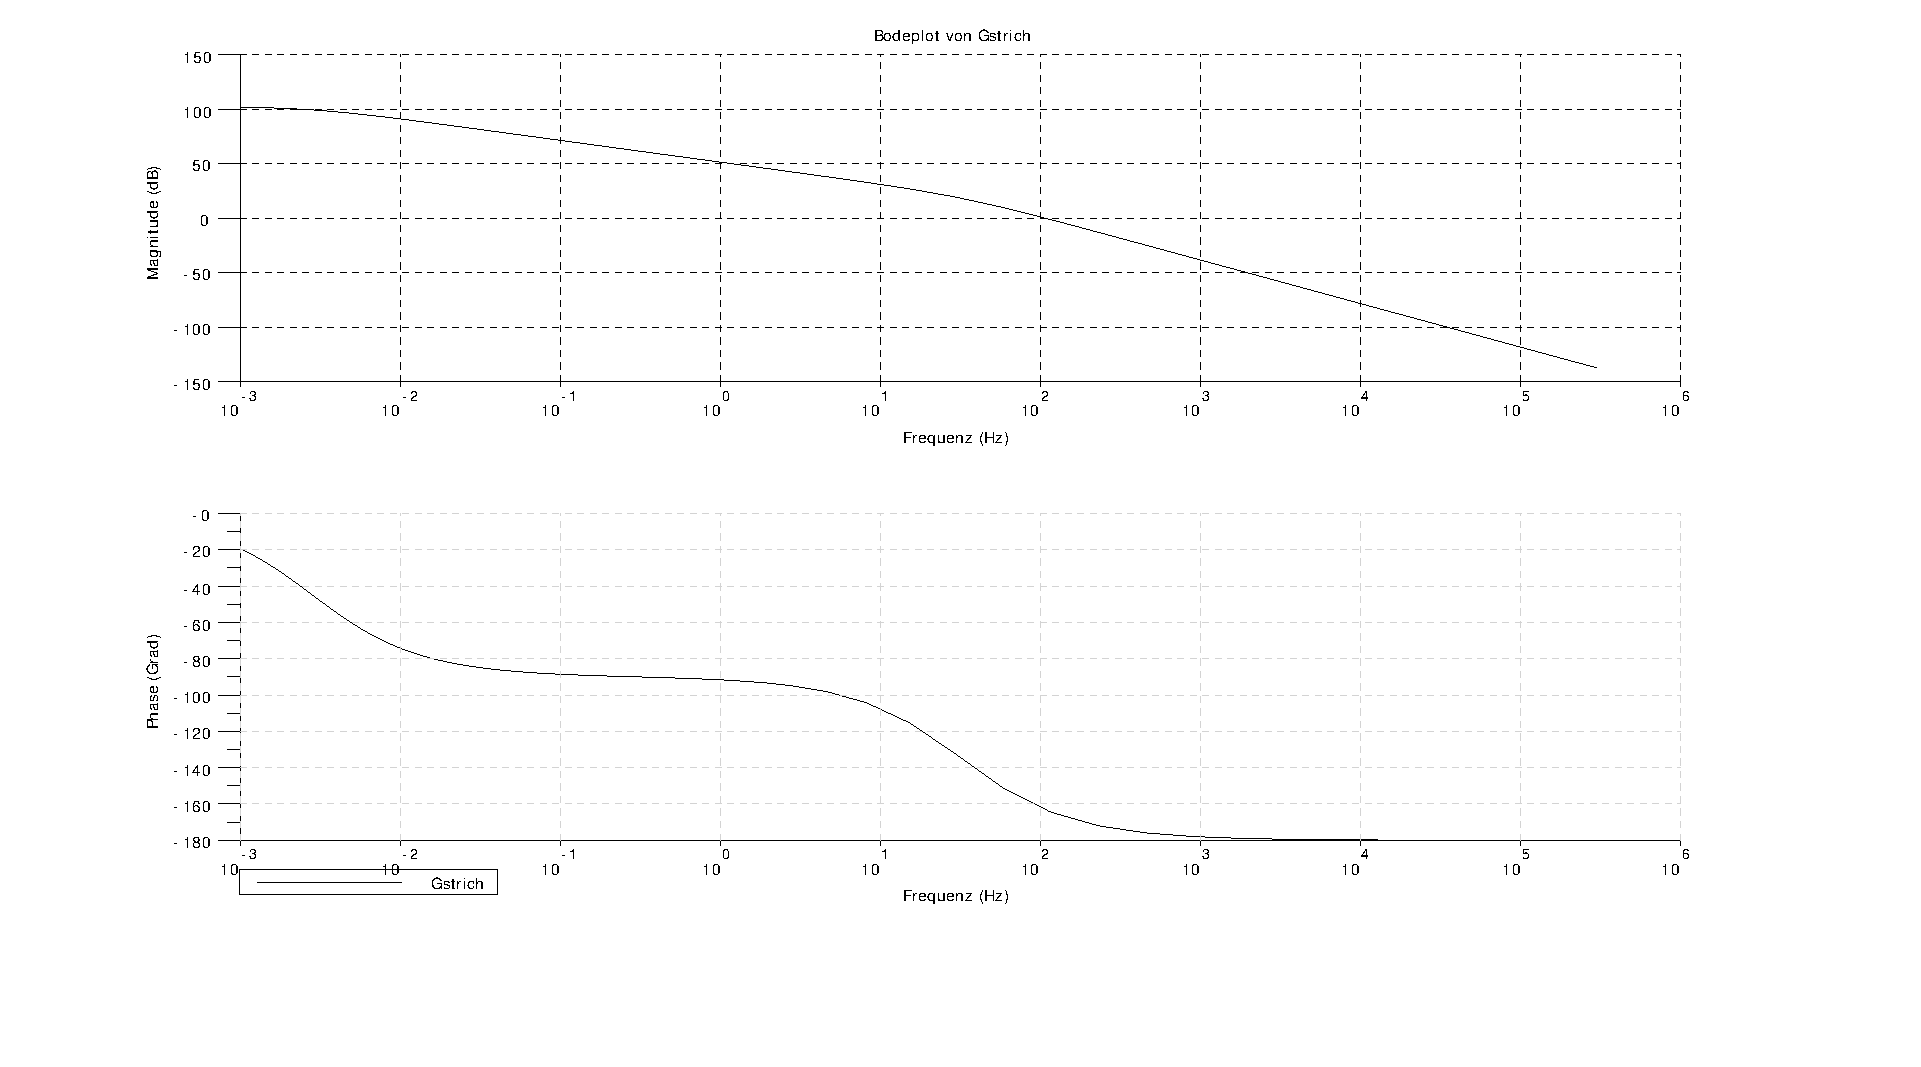
\includegraphics[scale=0.5, trim = 0cm 0cm 0cm 0cm, clip]{./Bilder/BodevonGstrich}
                    \caption{caption}
                    \label{fig:BodevonGstrich}
            \end{figure}
       
        \end{quote}

        \subsubsection{Reglerentwurf}
        Aufgabe:\\        
        Wählen Sie zunächst das aus der Vorlesung bekannte Entwurfsvorgehen, indem Sie mit der Nullstelle $s_{0,\omega}$
        des Reglers die langsamste Polstelle der Strecke kürzen. Bestimmen Sie dann mit Hilfe von Simulationen die
        Verstärkung $k_\omega$ so, dass der geschlossene Regelkreis eine Ausregelzeit von etwa $0.6$ Sekunden aufweist
        und das Ü̈berschwingen einen Wert von $20\%$ nicht übersteigt. Rufen Sie sich in Erinnerung, wie die
        Kenngrößen ``Überschwingweite'' , ``Ausregelzeit'' , ``Phasenreserve'' und ``Durchtrittsfrequenz''
        miteinander in Beziehung stehen!
        \begin{quote} 

            \vspace{1em}
            ``Überschwingweite'': Bei der Überschwingweite handelt es sich um die maximale Abweichung der Reglegröße vom
            Sollwert, $\Delta y = max(y) - y_{soll}$, nach dem die Relgröße die Sollgröße überschritten hat.
            \cite{Ueberschwingweite}\\
  
            
            \vspace{1em}
            ``Ausregelzeit'' : Die Ausregelzeit ist die Zeit bis die Regelgröße nach einer sprungförmigen Änderung der
            Führungs- oder Störgröße einen Toleranzbereich um den Sollwert erreicht und diesen Toleranzbereich anschließend
            nicht mehr verläßt.
            \cite{Ausregelzeit}\\

            
            \vspace{1em}
            ``Durchtrittsfrequenz'': Bei der Durchtrittsfrequenz handelt es sich um diejenige Frequenz bei der der
            Amplitudenfrequenzgang die $0dB$ Achse schneidet.\\

            \vspace{1em}
            ``Phasenreserve'': Die Phasenreserve ist der Abstand des Phasengangs zu $180^\circ$ auf höhe der Durchtrittsfrequenz.
            ($\varphi_R = 180^° - \varphi(\omega_D)$)\\
            
            
            \vspace{2em}
            Phasenreserve und Überschwingweite hängen folgendermaßen zusammen:\\
            \begin{equation*}
                \begin{split}
                \varphi_R [^\circ] + e_{max} [\%] \approx 70
                \end{split}
            \end{equation*}
            
            \vspace{1em}
            Auch Amplitudenreserve und Anstiegszeit hängen voneinander ab. Je kürzer die Anstiegszeit ist desto
            höher ist die maximale Überschwingweite und desto geringer ist auch die Amplitudenreserve. In
            der Praxis wird oft auch der Zusammenhang von Durchtrittsfrequenz und Anstiegszeit
            verwendet:
            \begin{equation*}
            \begin{split}
                \omega_D = \frac{1}{T_{a,50}} \p (1,5- \frac{e_{max} [\%]}{250})
            \end{split}
            \end{equation*}
            \cite{krachler}
        \end{quote}

		
		Zum Reglerentwurf:\vspace{1em}
		
		Das Bode-Diagramm des Reglers $K_2$ mit einer Verstärkung von $1$ und das resultierende Diagramm für $G_\omega^{'}
		K_2$ sehen folgendermaßen aus:
		\begin{figure}[H]
        \centering
            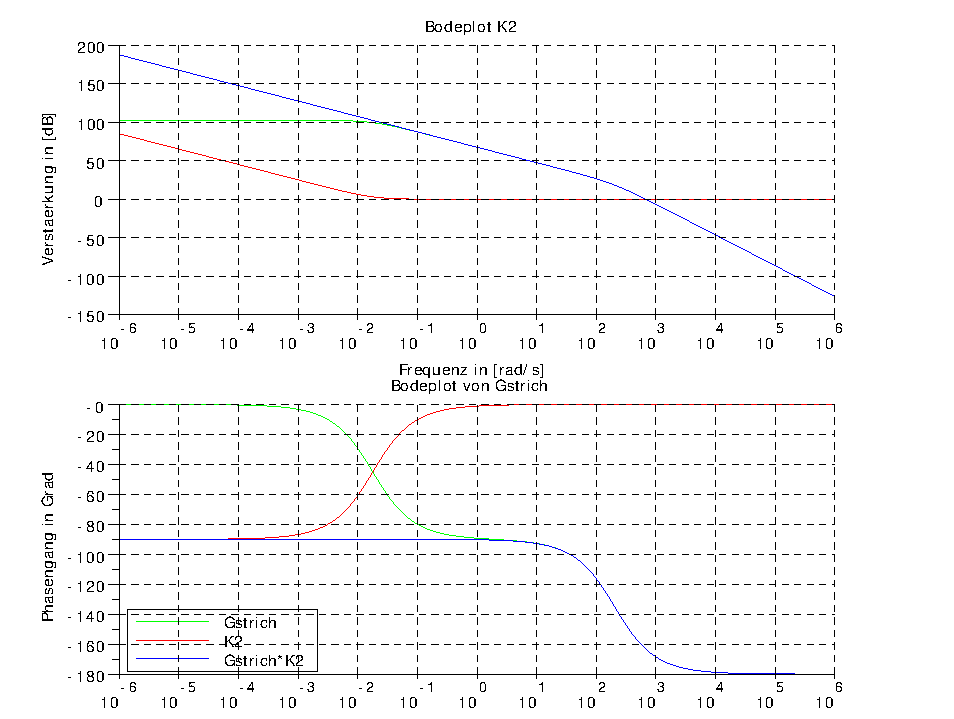
\includegraphics[scale=0.7, trim = 0cm 0cm 0cm 0cm, clip]{./Bilder/K2GstrichVersion1verstaerkung1}
                \caption{Bode-Diagramm Gstrich, K2 und Gstrich K2}
        \end{figure}
    
        Um unsere Anforderungen zu erfüllen, streben wir eine Phasenreserve von ca. $60^{\circ}$ an. Aus dem Bodediagramm
        wird ersichtlich, dass der Regler $K_\omega$ dazu eine Verstärkung von ca. $-20dB$ benötigt.\\
        Die Änderung der Verstärkung hat folgende Auswirkung auf den Bodeplot:
        \begin{figure}[H]
        \centering
            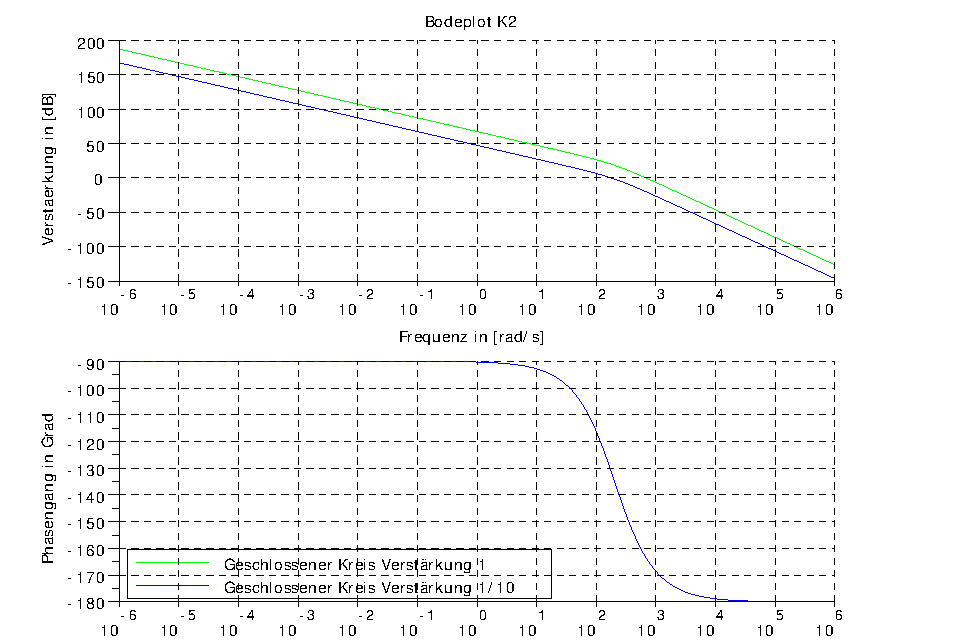
\includegraphics[scale=0.7, trim = 0cm 0cm 0cm 0cm, clip]{./Bilder/BodeGschlossenverstaerkt}
                \caption{Bodeplot geschlossener Kreis}
        \end{figure}
        
        Mit dieser Verstärkung ergibt sich folgende Sprungantwort:
        \begin{figure}[H]
        \centering
            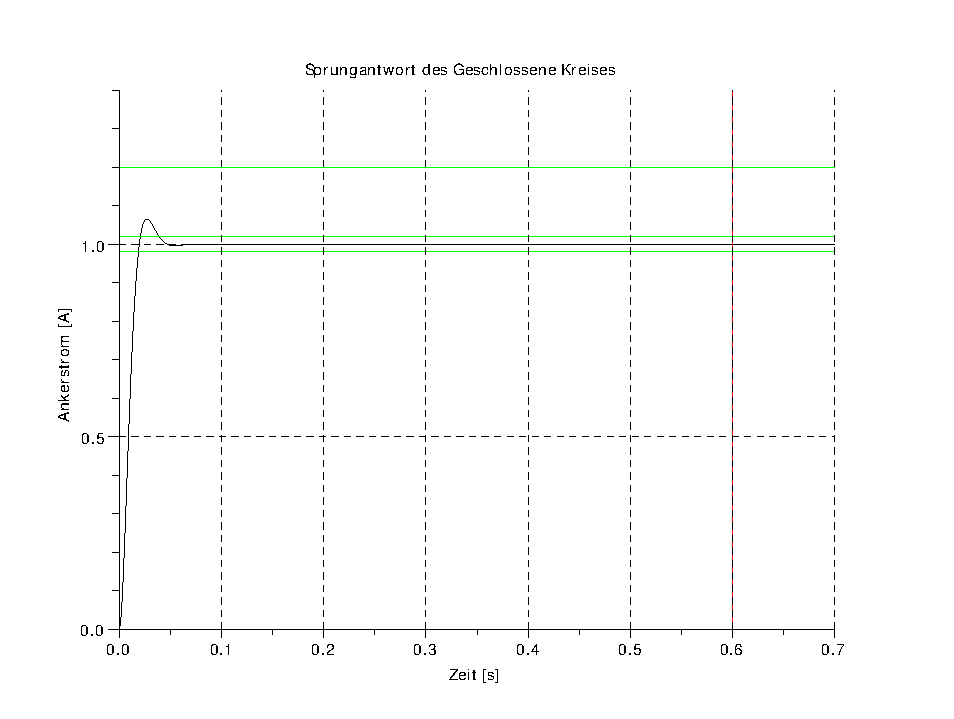
\includegraphics[scale=0.7, trim = 0cm 0cm 0cm 0cm, clip]{./Bilder/Sprungantwortlangsam}
                \caption{Sprungantwort}
        \end{figure}
        
        
        
        \subsubsection{Erstellen der Führungsübertragungsfunktion}
        \label{2d}
        Aufgabe:\\
        Bei Sprüngen der Führungsgröße $r_\omega$ von $0$ auf Werte bis zu $180 \frac{rad}{s}$ soll die Stellgrößenbeschränkung
        von $−5V < u < 5V$ nicht verletzt werden. Überprüfen Sie simulativ, ob Ihr Regler diese Forderung erfüllt. Falls nicht,
        korrigieren Sie ihre Reglerparameter, sodass die Forderung erfüllt wird.
        Wie lautet die Übertragungsfunktion $\overline{T}_\omega$ des bis hierhin entworfenen geschlossenen Regelkreises?
        \begin{quote}
            
            \begin{equation*}
            	\begin{split}
            		\overline{T}_\omega &= \frac{G_\omega^{'} K_\omega}{1 + G_\omega^{'} K_\omega}\\ \\
            		&= \frac{47555.923}{47555.923 + 202.22547 s + s^2}
            	\end{split}
            \end{equation*}
        \end{quote}
        
        \subsubsection{Erstellen der Störübertragungsfunktion}
        \label{2e}
        Aufgabe:\\
        Berechnen Sie die Störübertragungsfunktion $\overline{G}_{m\omega} (s) = \frac{\Omega(s)}{M_L (s)}$ vom
        Lastmoment $m_L$ auf die Winkelgeschwindigkeit $\omega$. Simulieren Sie die Störsprungantwort. Warum ist das
        Störverhalten des entworfenen Regelkreises nicht brauchbar? Was fällt Ihnen auf, wenn Sie die Pole von
        $\overline{T}_\omega$ und $\overline{G}_{m\omega}$ vergleichen?
		\begin{quote}
			\begin{equation*}
            	\begin{split}
            		\overline{G}_{m\omega} (s) &= \frac{\Omega(s)}{M_L (s)} = \frac{\frac{1}{km}G_{i\omega}}{1+ G_\omega^{'}
            		K_\omega}\\ \\
            		&= \frac{9023894.2s + 44622.936s^2}{848.83396 + 47559.532s + 202.24332s^2 + s^3}
            	\end{split}
            \end{equation*}
            
            Die Störsprungantwort sieht folgendermaßen aus:
            \begin{figure}[H]
                \centering
                    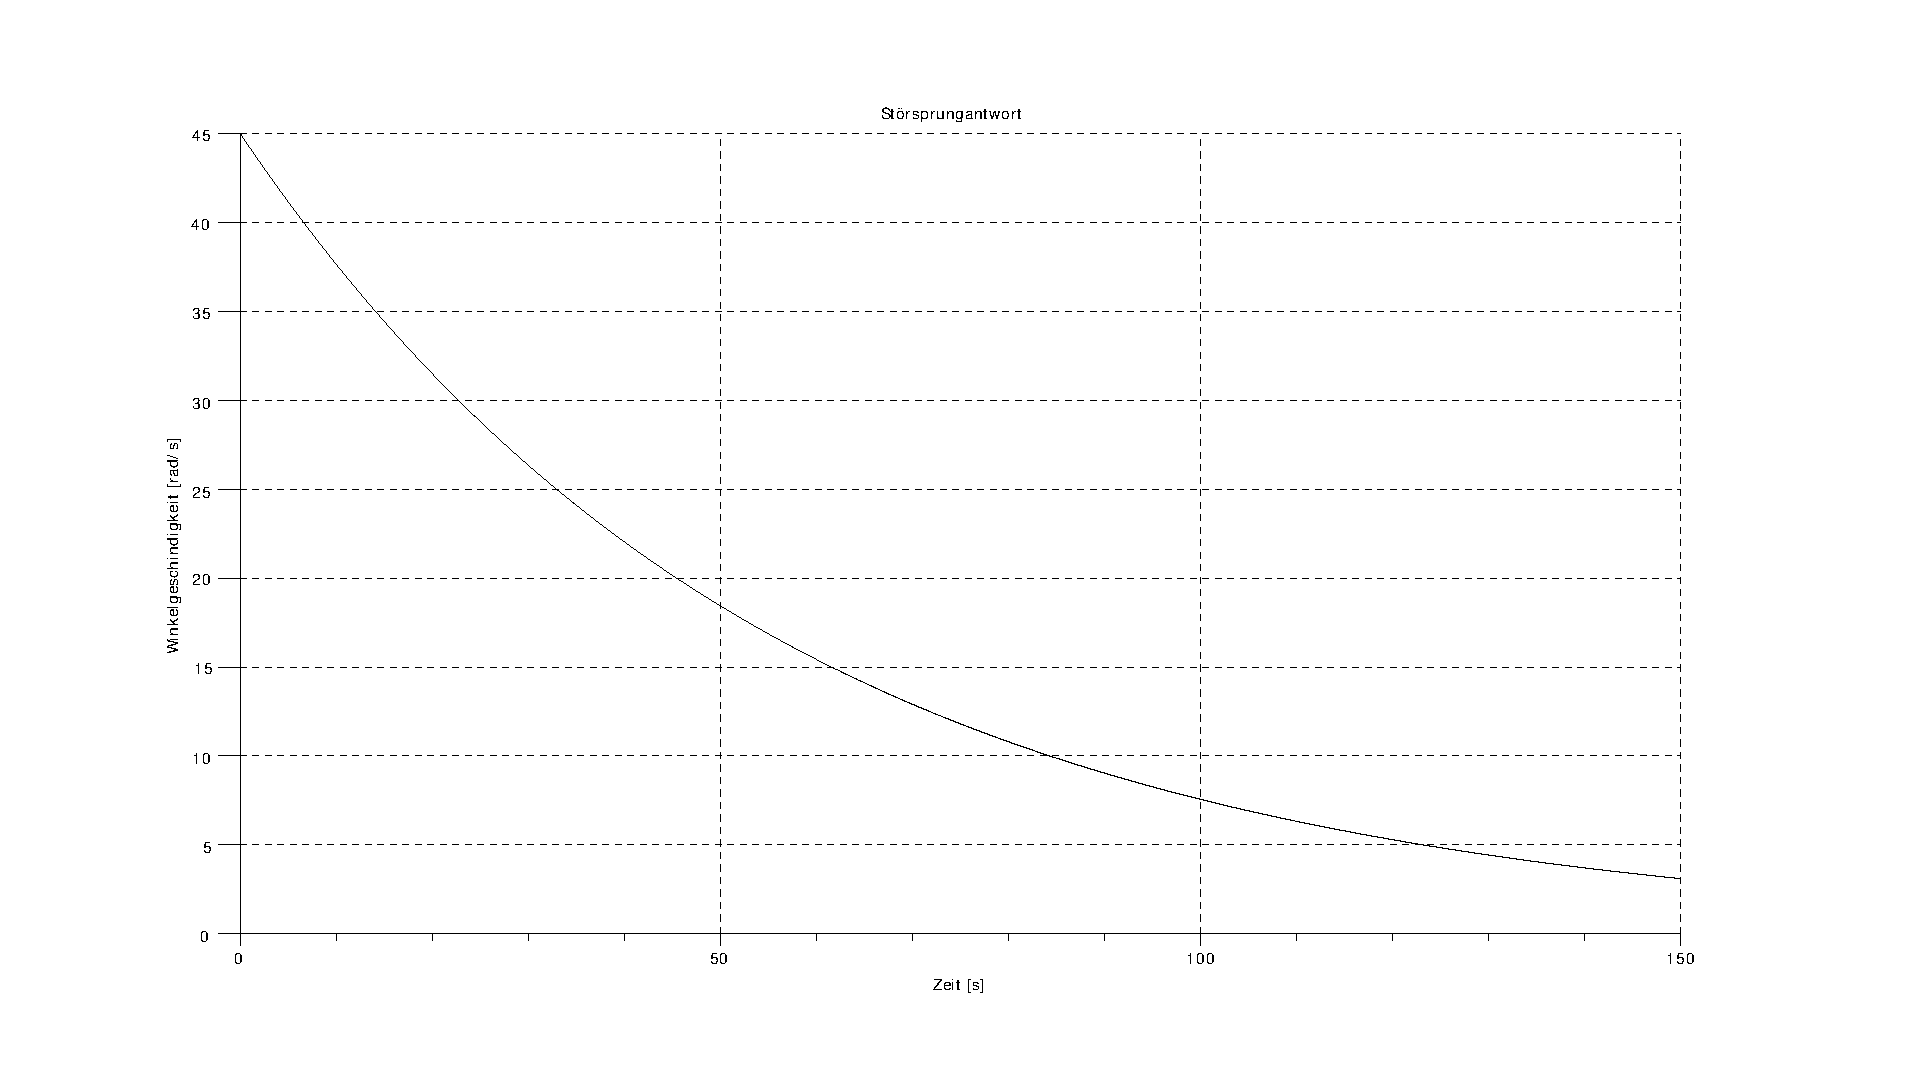
\includegraphics[scale=0.5, trim = 0cm 0cm 0cm 0cm, clip]{./Bilder/Stoersprungantwortlangsam}
                        \caption{Langsame Stoersprungantwort}
                        \label{fig:filename}
            \end{figure}
            
            Es fällt auf, dass die Störsprungantwort extrem langsam, und daher vermultich nicht zu gebrauchen ist. Selbst
            nach über \SI{150}{s} hat der Regler es, in der Simulation, nicht geschafft die Störung auszuregeln.\vspace{1em}
            
            Ob eine solch langsame Störsprungantwort zu gebrauchen ist hängt selbstverständlich von dem Problem ab für
            das der Regler entworfen werden soll. Da unsere Führungssprungantwort aber eine Ausregelzeit von $0,6s$
            aufweisen sollte und unsere Störsprungantwort eine Ausregelzeit größer als $150 s$ aufweist erfüllt
            dieser Regler nicht die Anforderungen.\vspace{1em}
            
            Beim Vergleichen der Polstellen von $\overline{T}_\omega$ und $\overline{G}_{m\omega}$ fällt auf, dass
            $\overline{G}_{m\omega}$ neben den zwei Polstellen von $\overline{T}_{m\omega}$ eine zusätzliche Polstelle hat.\\
            
            $\overline{T}_\omega$ hat die Polstellen:\\
            \begin{equation*}
                \begin{split}
                    pol \overline{T}_\omega (1) &= - 101.11273 + 193.21526i\\
                    pol \overline{T}_\omega (2) &= - 101.11273 - 193.21526i\\
                \end{split}
            \end{equation*}\\
            
             Während $\overline{G}_{m\omega}$ folgende Polstellen besitzt:\\
             
            \begin{equation*}
                \begin{split}
                    pol \overline{G}_{m\omega} (1) &= - 101.11273 + 193.21526i\\
                    pol \overline{G}_{m\omega} (2) &= - 101.11273 + 193.21526i\\
                    pol \overline{G}_{m\omega} (3) &= - 0.0178492\\
                \end{split}
            \end{equation*}
            
            Diese zusätzliche Postelle von $\overline{G}_{m\omega}$ ist die langsame Polstelle der Strecke
            $G_\omega^{'}$, die wir bei dieser Reglerentwicklung mit der Nullstelle des Reglers eliminieren wollten.\\
            In der Übertragungsfunktion des Geschlossenen Kreises kürzt sich die Nullstelle des Reglers mit der
            Postelle der Strecke. Deshalb taucht diese Polstelle nicht mehr als Polstelle von $\overline{T}_\omega$
            auf. Bei der Störübertragungsfunktion $\overline{G}_{m\omega}$ hingegen kürzt sich diese Polstelle nicht
            raus und beeinflusst die Störsprungantwort sehr negativ.\\
            
            
            Im folgenden wird allgemein gezeigt, wie sich bei der komplimentären Sensitivitätsfunktion Pole der Strecke
            mit Nullstellen des Reglers kürzen, bei Sörübertragungsfunktionen dieser Form jedoch erhalten bleiben.\\
            Der Regler $K$ und die Strecke $G$ seinen folgendermaßen dargestellt. Die Pole der Strecke in $N_G$ werden
            durch gleich viele Nullstellen im Regler in $Z_K$ kompensiert.
            \begin{equation*}
            	\begin{split}
            		K &= \frac{Z_K}{N_K}\\
            		G &= \frac{Z_G}{N_G}\\
            	\end{split}
            \end{equation*}
            
            Für die Sensitivitätsfunktion heißt das:
            
            \begin{equation*}
            	\begin{split}
                    T &= \frac{GK}{1+GK} = \frac{\frac{Z_K}{N_K} \frac{Z_G}{N_G}}{1 + \frac{Z_K}{N_K}
                    \frac{Z_G}{N_G}}\\
                    &= \frac{Z_G Z_K}{N_G N_K + Z_G Z_K}\\
                    &= \frac{Z_G}{N_K + Z_G}
            	\end{split}
            \end{equation*}
                        
            Die Pole und Nullstellen in $N_G$ und $Z_K$ kürzen sich raus.\\
            
            Für die Störübertragungsfunktion hingengen ergibt sich:
            \begin{equation*}
            	\begin{split}
            		G_{m\omega} &= \frac{G}{1 + GK} = \frac{\frac{Z_G}{N_G}}{1 + \frac{Z_K}{N_K}\frac{Z_G}{N_G}}\\
            		&= \frac{Z_G N_K}{N_G N_K + Z_G Z_K}
            	\end{split}
            \end{equation*}
            
            In diesem Fall fehlt die Nullstellen des Reglers im Zähler der Störübertragungsfunktion. Daher bleiben die
            Polstellen in $G_{m\omega}$ erhalten.
            
            
		\end{quote}
		
		\subsubsection{Korrektur der Führungs- und Störübertragungsfunktion}
		\label{2f}
		Aufgabe:\\
	    Überlegen Sie mit Hilfe der Wurzelortskurve, wie die Nullstelle $s_{0,\omega}$ des Reglers verschoben werden muss, um
	    das Störverhalten zu verbessern. Wählen Sie $s_{0,\omega}$ und $k_\omega$ neu, sodass alle vorher genannten
	    Forderungen an das Führungsverhalten weiterhin erfüllt werden. Wie lauten die neue
	    Führungsübertragungsfunktion $T_\omega$ und die neue Störübertragungsfunktion $G_{m\omega}$ und deren Pole?
		\begin{quote}
		\vspace{1em}
        Nun verschieben wir die Nullstelle weiter in den Negativen bereich, wodurch das neue $T_\omega$ und das neue $G_{m\omega}$ gleich
        viele Pole haben. Das liegt daran, dass bei $T_\omega$ kein Pol mehr eliminiert wird.\\
        Mit der Nullstelle $s_{0\omega}$ bei $-10$ und mit einer Verstärkung von $\frac{1}{45}$ ergibt sich folgende
        Störsprungantwort.
			
			\begin{figure}[H]
            \centering
                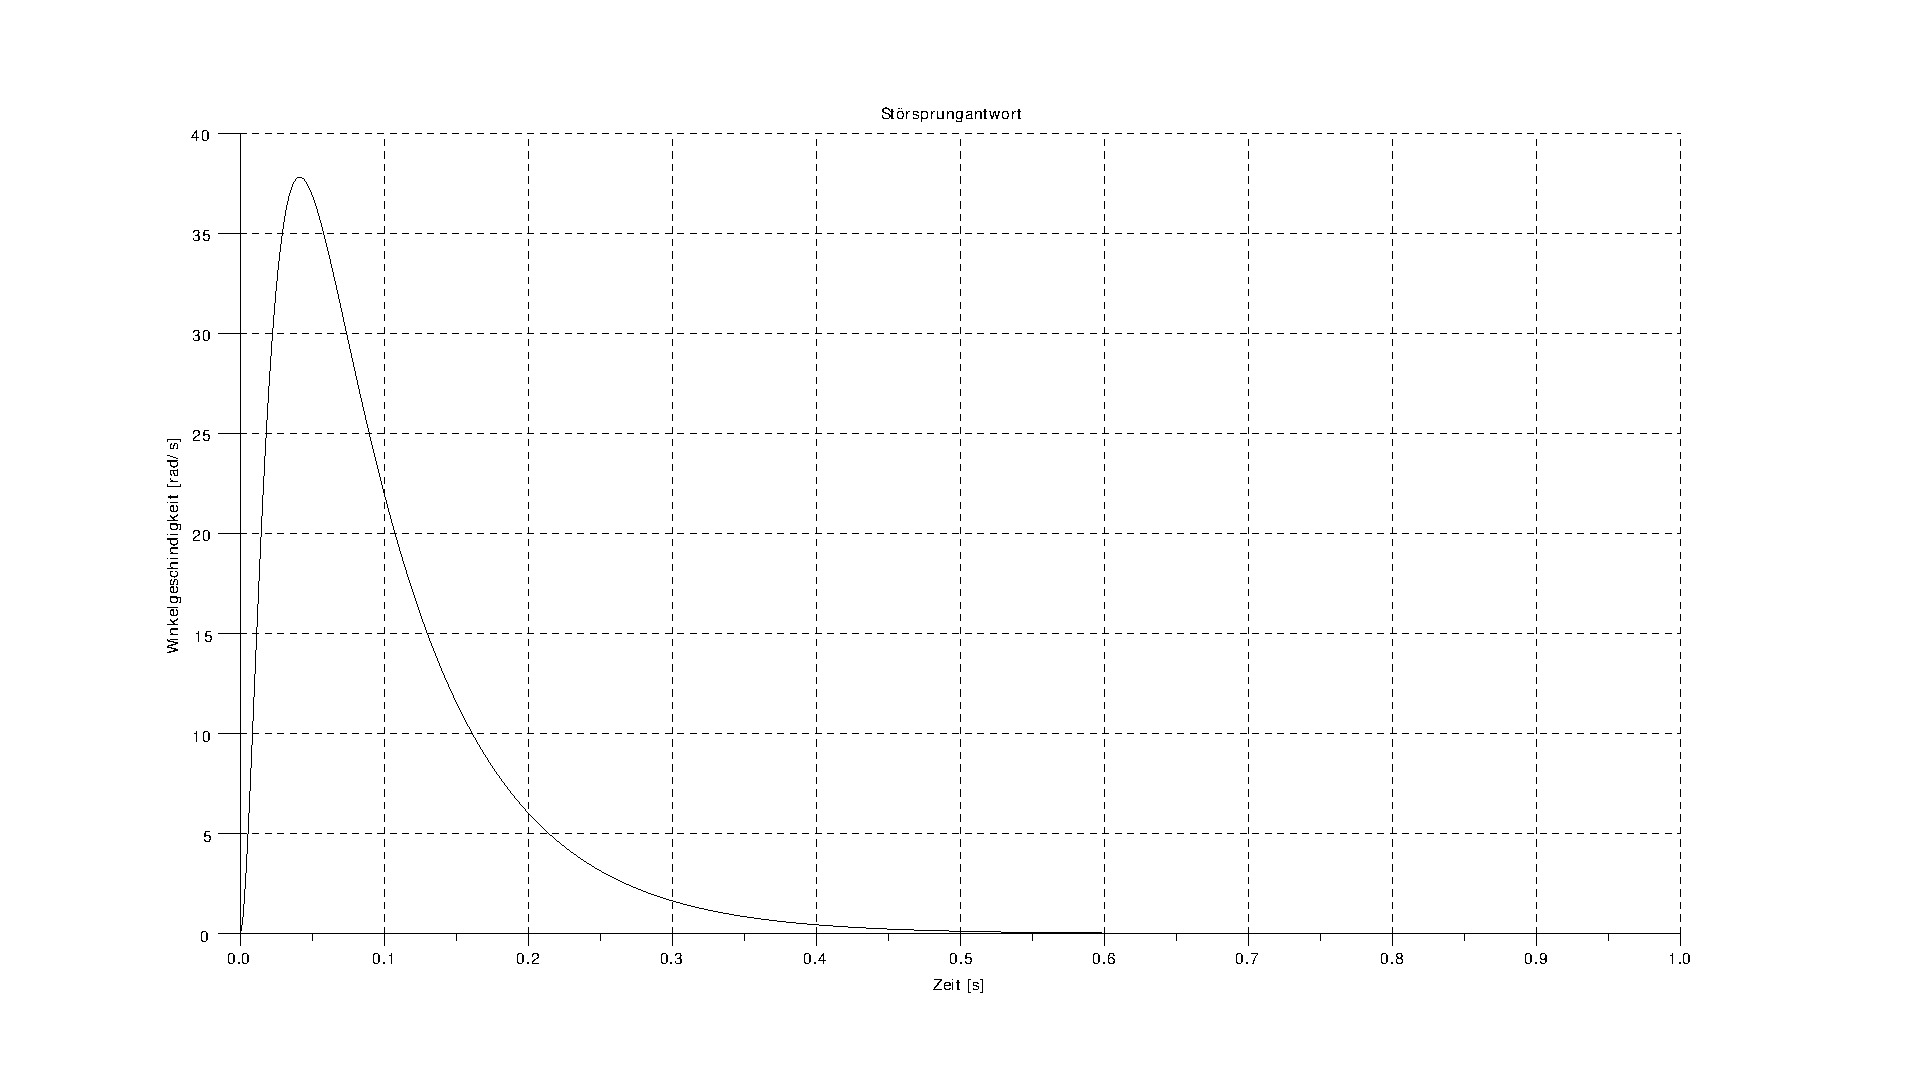
\includegraphics[scale=0.5, trim = 0cm 0cm 0cm 0cm, clip]{./Bilder/Stoersprungantwortschnell}
                    \caption{schnelle Störsprungantwort}
                    \label{fig:Stoersprungantwortschnell}
            \end{figure}
            
            Diese Störsprungantwort hat eien Ausregelzeit von $0,5s$ und reagiert damit um Größenordnungen schneller
            als bei unserer ersten Reglerentwicklung.\vspace{1em}
            
            Auch die Sprungantwort erfüllt mit diesen Werten alle Bedingungen:
            \begin{figure}[H]
            \centering
                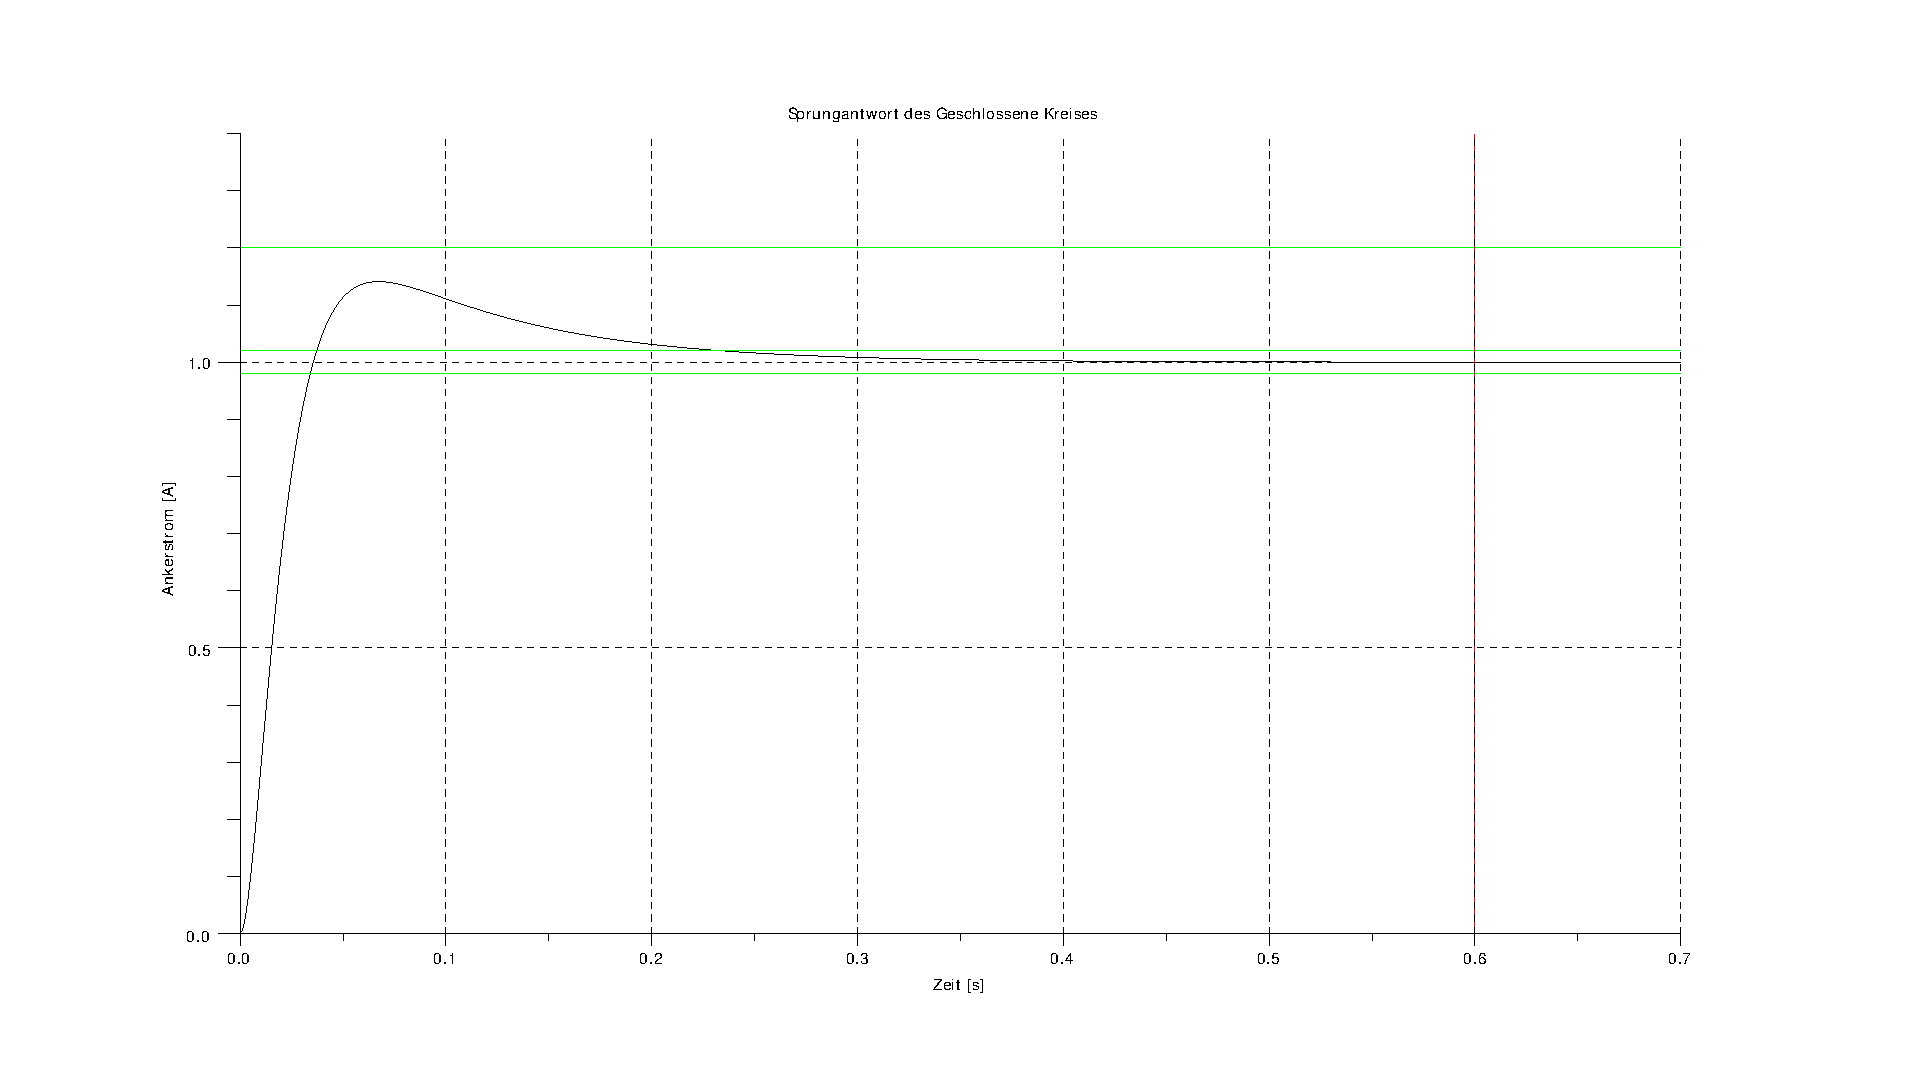
\includegraphics[scale=0.5, trim = 0cm 0cm 0cm 0cm, clip]{./Bilder/Sprungantwortschnell}
                    \caption{Sprungantwort}
                    \label{fig:./Bilder/Sprungantwortschnell}
            \end{figure}
    
    
            Die aus diesen Voraussetzungen entstehenden Übertragungsfunktionen $T_\omega$ und $G_{m\omega}$ lauten:\\
            
            \begin{equation*}
            	\begin{split}
            		T_\omega = \frac{105679.83 + 10567.983s}{105679.83 + 10571.592s + 202.24332s^2 + s^3}\\ \\
            		G_{m\omega} = \frac{9023894.2s + 44622.936s^2}{105679.83 + 10571.592s + 202.24332s^2 + s^3}
            	\end{split}
            \end{equation*}\\
            
            Am selben Nenner von $T_\omega$ und $G_{m\omega}$ lässt sich erkennen, dass die beiden Übertragungsfunktionen die
            Selben Polstellen besitzen.\\
            
            $T_\omega$ hat die Polstellen:\\
            
            \begin{equation*}
                \begin{split}
                    pol T_\omega (1) &= - 123.67194\\
                    pol T_\omega (2) &= - 65.531604\\
                    pol T_\omega (3) &= - 13.039776\\                   
                \end{split}
            \end{equation*}\\
            
            Während $G_{m\omega}$ folgende Polstellen besitzt:\\
            
            \begin{equation*}
                \begin{split}
                    pol G_{m\omega} (1) &= - 123.67194\\
                    pol G_{m\omega} (2) &= - 65.531604\\                
                    pol G_{m\omega} (3) &= - 13.039776\\              
                \end{split}
            \end{equation*}
            
		\end{quote}
		
	\end{quote}
	
	\subsection{Anti-Windup-Schaltung in Scicos erstellen}
	Aufgabe:\\
    Erweitern Sie Ihre Reglerstruktur in Scicos um eine Anti-Windup-Schaltung. Beziehen Sie sowohl
    den äußeren als auch den inneren Regler in die Schaltung ein. Realisieren Sie dafür den inneren und äußeren
    PI-Regler in einer Parallelform mit P- und I-Anteil.
	\begin{quote}
		
		
	\end{quote}
	
\end{quote}

%--------------------------------------------------------------------
%--------------------------------------------------------------------

\section{Durchführung}
\begin{quote}
    
    
    \subsection{Regler mit guten Störeigenschaften}
    Implementieren Sie ihre Kaskadenregelung mit innerem und äußerem Regler und der
    Anti-Windup-Schaltung in Scicos und erstellen Sie mit dem Betreuer das echtzeitfähige
    Programm zur Motoransteuerung. Verwenden Sie für den äußeren Regler zunächst die
    Parameter aus Aufgabe \ref{2f}.
    
    
    \begin{quote}
        
        \subsubsection{Führungssprungantwort}
        Nehmen Sie die Führungssprungantwort des Drehzahlregelkreises auf. Schalten Sie dafür den Sollwert der
        Winkelgeschwindigkeit von $0 \mathrm{\frac{rad}{s}}$ auf $150 \mathrm{\frac{rad}{s}}$ Nehmen Sie zusätzlich zu der
        Regelgröße auch die Stellgröße $r_i$ des Regelkreises auf.
        Beschreiben und diskutieren Sie das Regelkreisverhalten! Vergleichen Sie das Ergebnis mit der Simulation des
        Führungsverhaltens aus der Vorbereitungsaufgabe \ref{2f}!
        
        \begin{quote}
            
        \begin{center}
        \begin{tabular}{ll}
        
        \hspace{-4.5cm}
            \begin{minipage}{0.6\textwidth}
                
                \begin{figure}[H]
                    \label{fig:sprung_w}
                    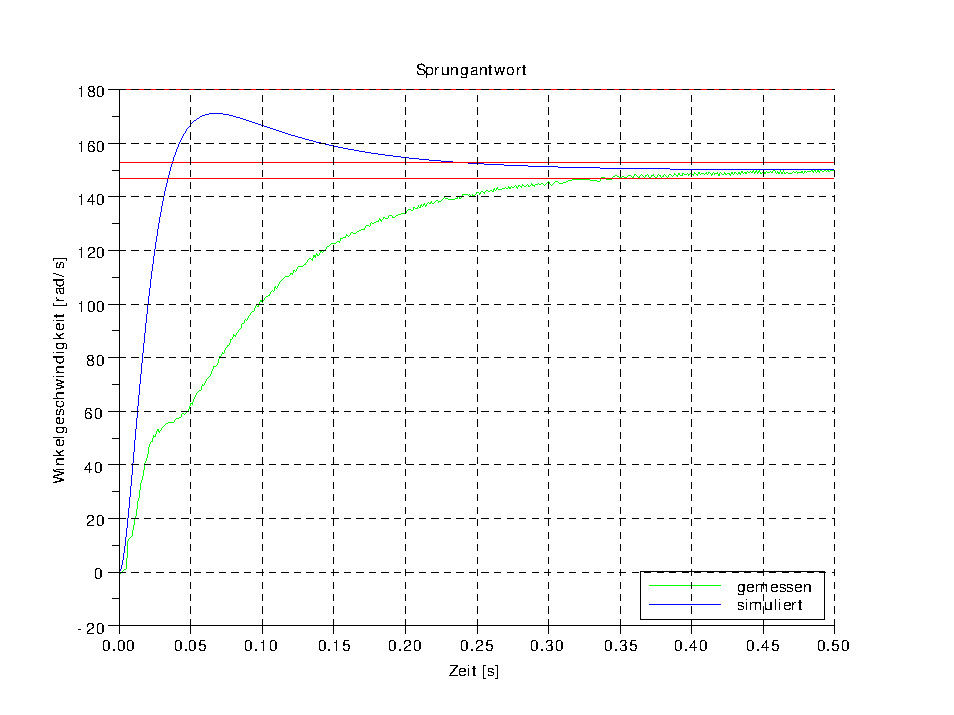
\includegraphics[scale=0.7, trim = 8mm 5mm 15mm 10mm, clip]{Bilder/sprung_w}
                    \caption{Sprungantwort der Winkelgeschwindigkeit}
                \end{figure}
                
            \end{minipage}
            
            \begin{minipage}{0.6\textwidth}
                \begin{figure}[H]
                    \label{fig:sprung_i}
                    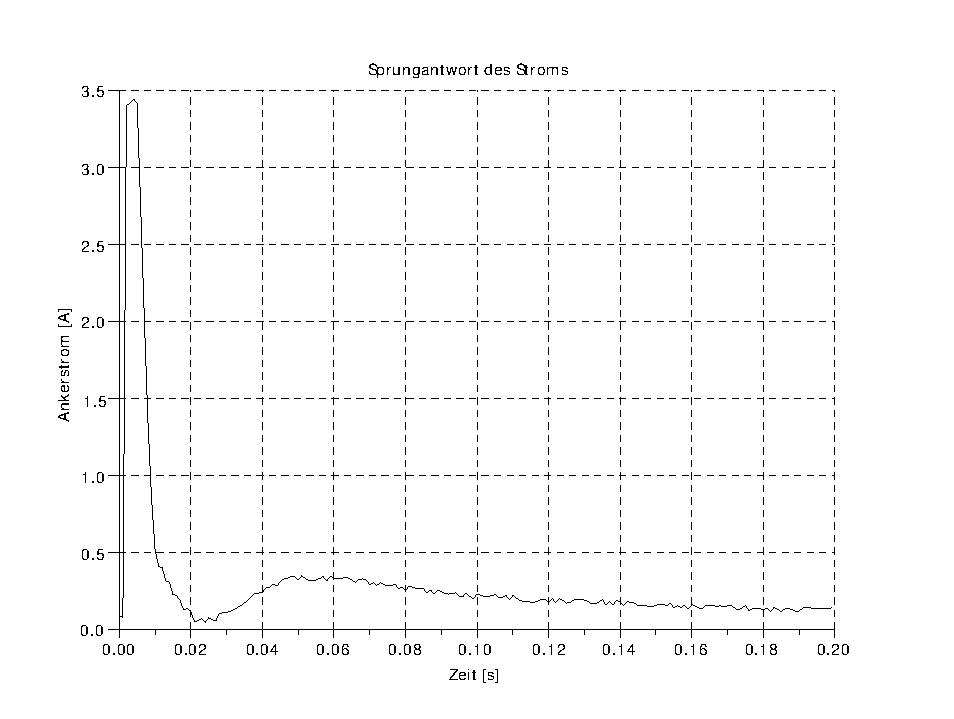
\includegraphics[scale=0.7, trim = 8mm 5mm 15mm 10mm, clip]{Bilder/sprung_i}
                    \caption{Sprungantwort des Stroms}
                \end{figure}
                
            \end{minipage}
            
        \end{tabular}
        \end{center}
        
        \vspace{2em}
        
        Die Sprungantworten erfüllen alle gestellten Bedingungen. Die Geschwindigkeit ändert sich etwas langsamer als
        simuliert, erreicht jedoch schon nach \si{0,35}{s} den angestrebten Wert von $150 \mathrm{\frac{rad}{s}}$. Die geringe
        Abweichung ist mit höherer Trägheit und mehr Reibmoment gegenüber der Simulation zu erklären.\\
        Auch die Sprungantwort des Stroms stellt sich mit nur geringem Überschwingen sehr schnell wieder ein.
        
        
        
        \end{quote}
        
        
        \subsubsection{Störsprungantwort}
        Nehmen Sie die Störsprungantwort des Systems auf. Betreiben Sie den Motor bei einer Winkelgeschwindigkeit von $150
        \mathrm{\frac{rad}{s}}$ und lösen Sie die Rückhaltevorrichtung der Bremse um ein sprunghaftes Lastmoment zu erhalten.
        Nehmen Sie zusätzlich zu der Regelgröße auch die Stellgröße $r_i$ des Regelkreises auf. Beschreiben und diskutieren Sie
        das Regelkreisverhalten! Vergleichen Sie das Ergebnis mit der Simulation des Störverhaltens aus der Vorbereitungsaufgabe
        \ref{2f}!
        
        \begin{quote}
            
        \begin{center}
        \begin{tabular}{ll}
        
        \hspace{-4.5cm}
            \begin{minipage}{0.6\textwidth}
                
                \begin{figure}[H]
                    \label{fig:stoersprung_w}
                    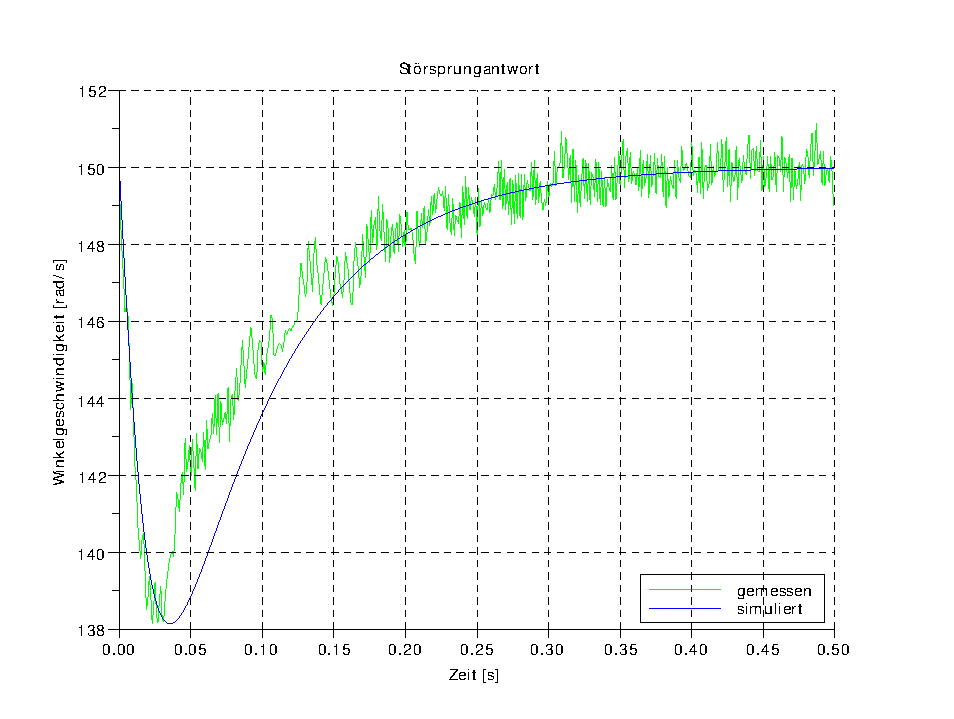
\includegraphics[scale=0.7, trim = 8mm 5mm 15mm 10mm, clip]{Bilder/stoersprung_w}
                    \caption{Störsprungantwort der Winkelgeschwindigkeit}
                \end{figure}
                
            \end{minipage}
            
            \begin{minipage}{0.6\textwidth}
                \begin{figure}[H]
                    \label{fig:stoersprung_i}
                    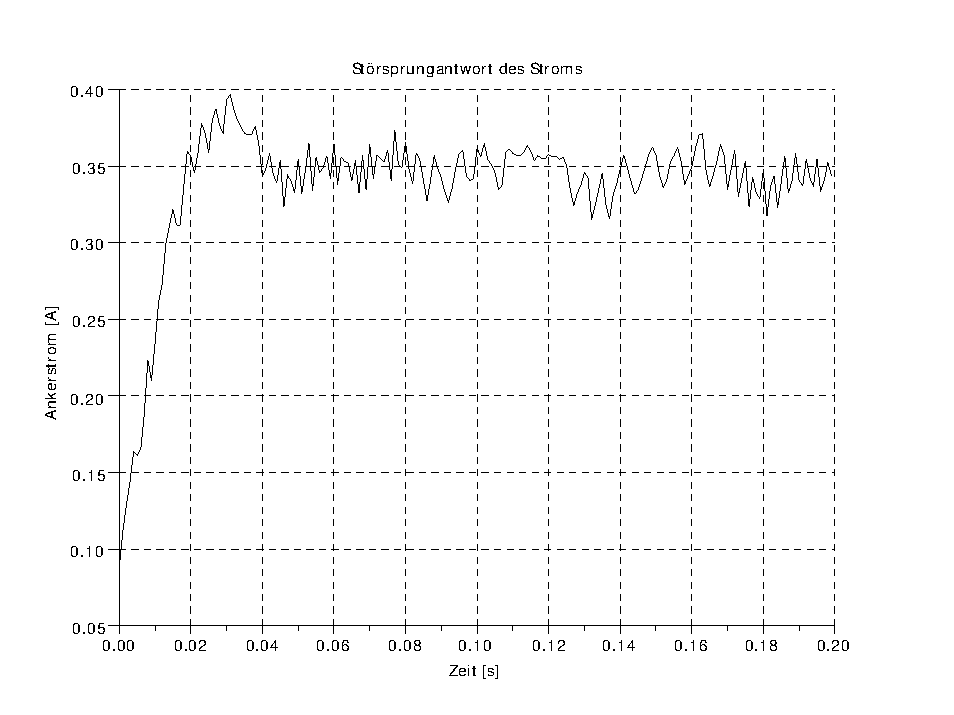
\includegraphics[scale=0.7, trim = 8mm 5mm 15mm 10mm, clip]{Bilder/stoersprung_i}
                    \caption{Störsprungantwort des Stroms}
                \end{figure}
                
            \end{minipage}
            
        \end{tabular}
        \end{center}
        \vspace{2em}
        
        Wie auch schon bei letzten Versuch beobachtet reagiert die Störsprungantwort des Reglers sogar etwas schneller als wir es
        simuliert haben. Dies hängt wiederum mit ungenauigkeiten der Realen bauteile zusammen, welche sich in diesem Fall zu
        unseren Gunsten auswirken.\\
        Der Störsprung des Stroms ist auch sehr gut. Der Strom stellt sich mit sehr geringem Überschwingen schon nach nur
        \si{0,04}{s} auf seinen neuen Wert von ca. \si{350}{mA} ein.
        
        
        \end{quote}
    
    \end{quote}
    
    
    \subsection{Regler mit schlechten Störeigenschaften}
    Untersuchen Sie nun den Regelkreis mit den zuerst bestimmten Parametern aus Aufgabe
    \ref{2d}. Nehmen Sie die Störsprungantwort des Systems auf. Wie äußert sich das unbefriedigende Störverhalten in der Praxis?
    Vergleichen Sie das Ergebnis mit der Simulation des Störverhaltens aus der Vorbereitungsaufgabe \ref{2e}!
    
    \begin{quote}
        
        Dieser Versuchsteil hat leider nicht den gewünschten bzw. erwarteten Erfolg gebracht. Erwartet hätten wir einen
        ähnlich schnelle Führungssprungantwort wie mit dem guten Regler jedoch eine sehr viel langsamere
        Störsprungantwort. Der Versuch hat jedoch schon eine sehr langsame Führungssprungantwort, mit
        einer Ausregelzeit weit größer als $20 s$, ergeben. Laut unserer Simulation hätte sich hingegen eine Ausregelzeit von
        unter $0.1 s$ einstellen sollen. Den Fehler für diese Abweichung konnten wir nicht identifizieren.\vspace{1em}
        
        Unerklärlich war außerdem, dass die Änderung des Vorzeichens in der Rückführung des PT1-Gliedes im Scicos Modell
        keine Auswirkung auf das Regelverhalten hatte.\vspace{1em}
        
        Da wir leider keine vernünftigen Messergebnisse von diesem Versuch haben können wir weder etwas plotten noch
        analysieren.
        
        
    \end{quote}
    
    
    \subsection{Test der Anti-Windup-Schaltung}
    Testen Sie ihre Anti-Windup-Schaltung mit den Parametern aus Aufgabe \ref{2f}. Betreiben Sie den Motor bei einer
    Winkelgeschwindigkeit von $150 \mathrm{\frac{rad}{s}}$ und halten Sie die Scheibe sehr kurz fest um sie danach sofort wieder
    freizugeben. Wiederholen Sie den Versuch mit deaktivierter Anti-Windup-Schaltung! Nehmen Sie neben der Winkelgeschwindigkeit
    und dem Ankerstrom die Stellgrößen vor und nach der Beschränkung auf. Beschreiben und vergleichen Sie das Regelkreisverhalten
    mit und ohne Anti-Windup-Schaltung!
    
    \begin{quote}
        
        Bei diesem Versuch haben wir den laufenden Motor nicht nur durch eine Last in seiner Umdrehung gestört sondern ihn durch
        festhalten der Schwungscheibe kurz angehalten. Dadurch haben wir den Regler gezwungen so stark auf diese Störung zu
        reagieren, dass er mit seiner inneren Stellgröße $u$ in die Begrenzung von \si{\pm5}{V} geht. Diesen Versuch haben wir
        sowohl mit eingeschalteter als auch mit ausgeschalteter Wind-up Schaltung durchgeführt.\\
        Die Messergebniss der zwei Versuche sehen Folgendermaßen aus:

        \begin{figure}[H]
        \centering
            \label{fig:w}
            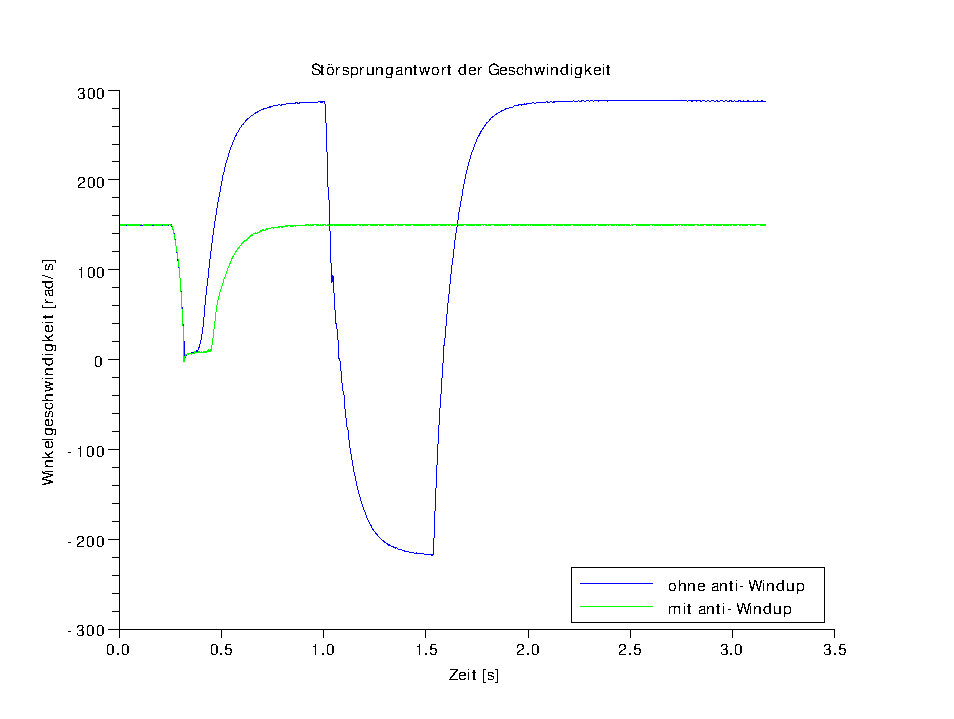
\includegraphics[scale=0.8, trim = 0.5cm 0.5cm 2cm 0.5cm, clip]
            {./Bilder/windup_sprungantwort_Geschwindigkeit}
            \caption{Störsprungantwort der Geschwindigkeit}
        \end{figure}
        
        \begin{figure}[H]
        \centering
            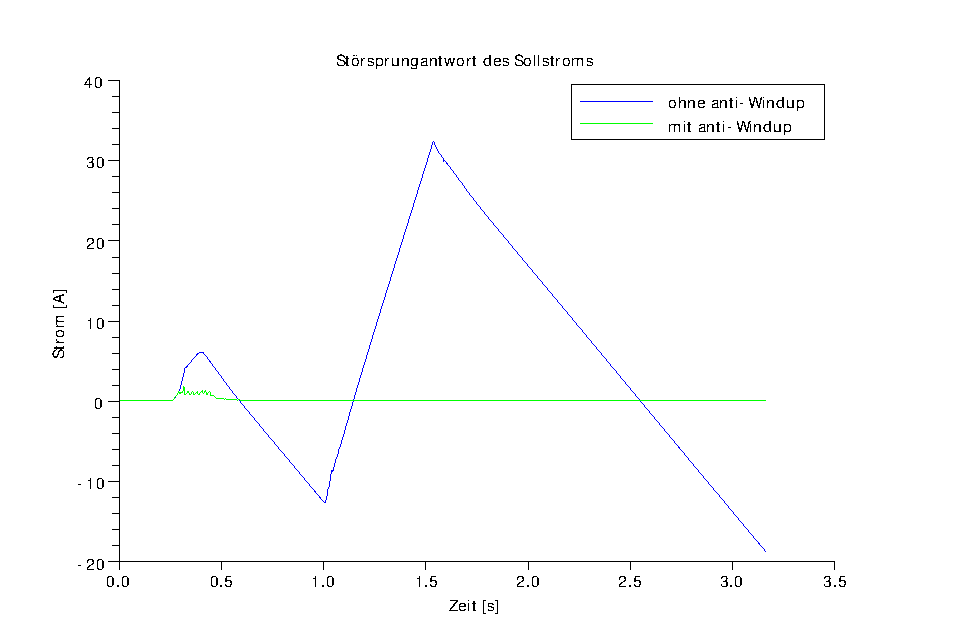
\includegraphics[scale=0.8, trim = 0.5cm 0.5cm 2cm 0.5cm, clip]
            {./Bilder/windup_sprungantwort_sollstrom}
            \caption{Störsprungantwort des Sollstroms}
        \end{figure}
        
        \begin{figure}[H]
        \centering
            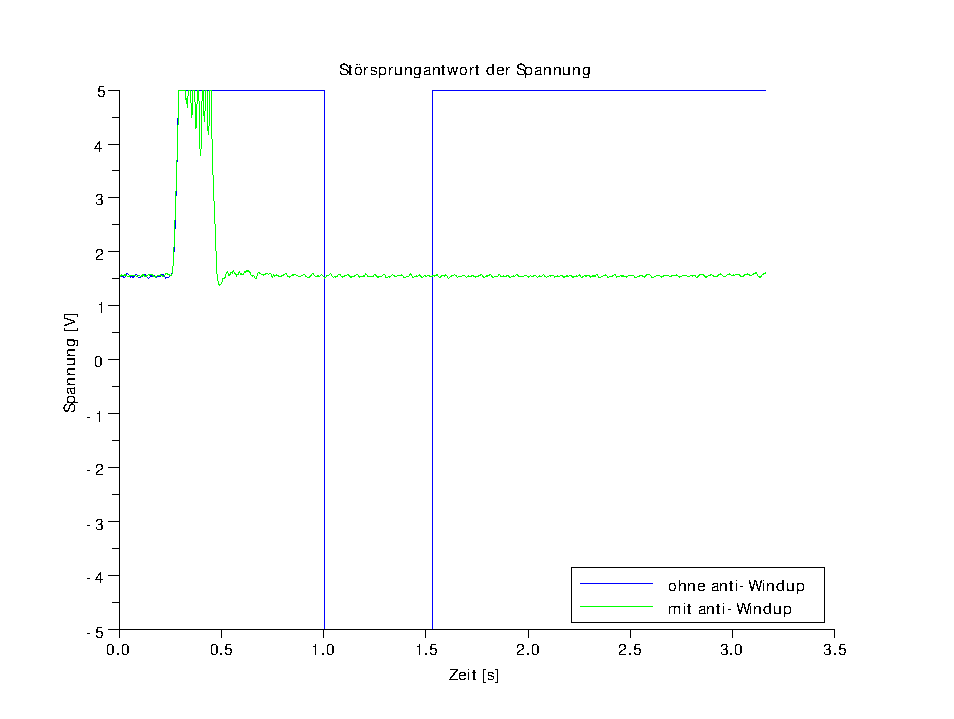
\includegraphics[scale=0.8, trim = 0.5cm 0.5cm 2cm 0.5cm, clip]
            {./Bilder/windup_sprungantwort_Spannung}
            \caption{Störsprungantwort der Spannung}
        \end{figure}
        

        \begin{figure}[H]
        \centering
            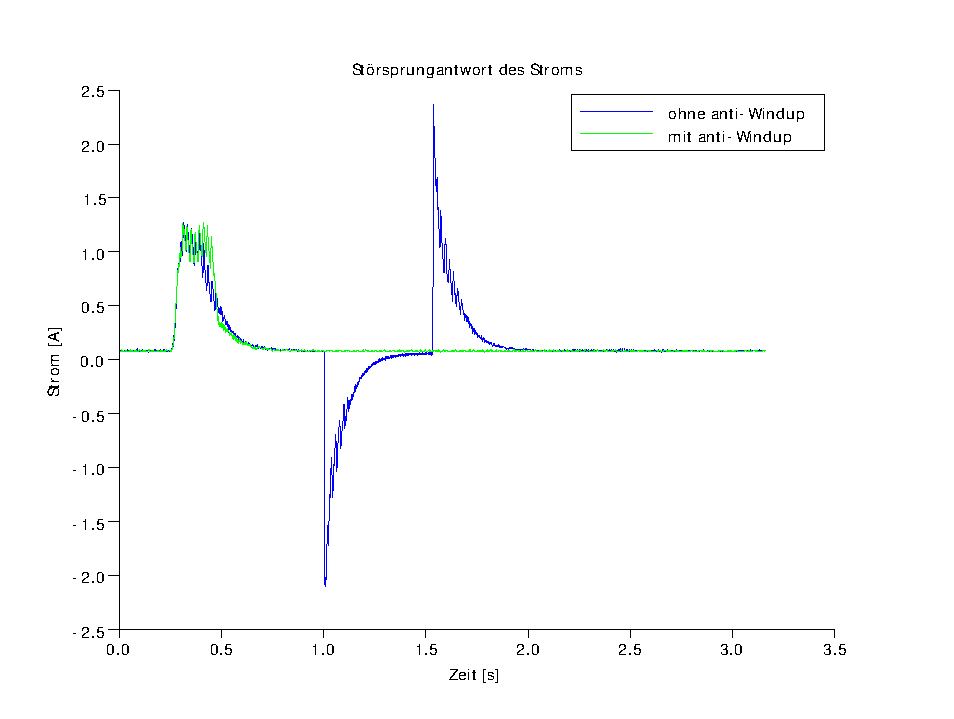
\includegraphics[scale=0.8, trim = 0.5cm 0.5cm 2cm 0.5cm, clip]
            {./Bilder/windup_sprungantwort_Strom}
            \caption{Störsprungantwort des Stroms}
        \end{figure}
        
        In der Grafik \ref{fig:w} sieht man klar, wann die Schwungscheibe 
        von $150 \frac{rad}{s}$ auf $0\frac{rad}{s}$ abgebremst wird. Als reaktion darauf versucht
        der Regler den Motor anzuregen. Dazu steigt der Sollstrom an, weshalb wiederum die Spannung sprungartig
        ansteigt. Hierbei wiederum gerät die Spannung in die Begrenzung.\\
        
        \subsubsection{aktive anti-Windup Schaltung}
		\begin{quote}
            Im Falle der aktivierten anti-Wind-up Schaltung bremst diese sofort die Intregratoren der beiden
            Stellgrößen, sodass nicht über die physikalische Beschränkung hinaus integriert wird. Dadurch stimmen die
            physikalischen Größen und die Stellgrößen weiterhin überein. Dies verhindert, dass die Regler mit ihren Reglgrößen
            über ihr Ziel hinausschießen.\\
            Dieser Effekt lässt sich sehr gut an den Grünen Linien in der Sprungantwort der Spannung sowie der
            Sprunganwort des Sollstroms erkennen.\\
            Auch an der Drehgeschwindigkeit lässt sich dieses abbremsen erkennen, da die Grüne Linie langsamer aus der
            Störung rauskommt als die Blaue. Dafür schafft sie es jedoch, sobald die gewünschte Drehzahl erreicht ist, die
            Beschleunigung komplett abzubremsen und hat somit die Störung ausgeregelt.\vspace{1em}
			
		\end{quote}
		
		\subsubsection{deaktive anti-Winfup Schaltung}
		\begin{quote}
            Im Gegensatz dazu versucht der Regler ohne anti-Windup die Störung auszugleichen als ob es keine Begrenzung gäbe. Das
            wiederum hat zur Folge, dass der Regler annimmt der Ankerstrom würde nicht ausreichen um gegenzusteuern und
            deshalb die Stellgröße weiter aufintegriert.\\
            Sobald der Regler sich der angestrebten Winkelgeschwindigkeit nähert, müsste er anfangen gegenzusteuern um 
            Überschwingen zu vermeiden. Da der Integrator des inneren Reglers inzwischen aber einen sehr hohen Wert angenommen
            hat, hat das gegensteuern zwar einen Einfluss auf den Integrator bzw. die theoretische Stellgröße, nicht jedoch auf
            die physikalische.\\
            Durch das fehlende Gegensteuern schwingt die Regelgröße über. Der Regler benötigt somit, falls er es überhaup schafft,
            sehr lange um die ursprüngliche Störung auszuregeln.\\
            Das Überschwingen lässt sich in allen vier Messerten erkennen.
		\end{quote}
        
    \end{quote}


    
    
    
    
\end{quote}

%--------------------------------------------------------------------
%--------------------------------------------------------------------



% \begin{quote}
%     \lstinputlisting[
%         caption={Scilab-script},
%         label=lst:scilab]
%         {./Scilab/Motor.sce}
%         
% \end{quote}

%--------------------------------------------------------------------
%--------------------------------------------------------------------
\begin{thebibliography}{999}
\bibitem {Ueberschwingweite} Prof. Dr.-Ing. Raisch, Jörg; Dipl.-Ing. Hess, Anne-Katrin; Dipl.-Ing. Seel, Thomas:
Grundlagen der Regelungstechnik - 4.Praktikum, S.5
\bibitem {Ausregelzeit} Prof. Dr.-Ing. Raisch, Jörg; Dipl.-Ing. Hess, Anne-Katrin; Dipl.-Ing. Seel, Thomas:
Grundlagen der Regelungstechnik - 4.Praktikum, S.5

%\usepackage{url}


\bibitem{krachler}Christian Krachler:
\href{http://www.krachler.com/fileadmin/user_upload/arbeiten/Reglersynthese_Christian_Krachler.pdf}{Reglersynthese nach dem Frequenzkennlinienverfahren}, S16, S22, 08.05.2012

%http://krachler.com/fileadmin/user\_upload/arbeiten/Reglersynthese\_Christian\_Krachler.pdf


%Name, Vorname.; evtl. Name2, Vorname2.: Titel des Dokumentes
%oder Buches, Zeitschrift/Verlag/URL (Auflage, Erscheinungsort, -jahr), ggf. Seitenzahlen
%\bibitem [Wiki10] {DigitaleMesskette2} \url{www.wikipedia.org}, Zugriff 22.03.2010
\end{thebibliography}


\end{document}
